% Example 

%%%%%%%%%
% Purpose

\def\keradius{
\begin{figure}[h]
    \centering
    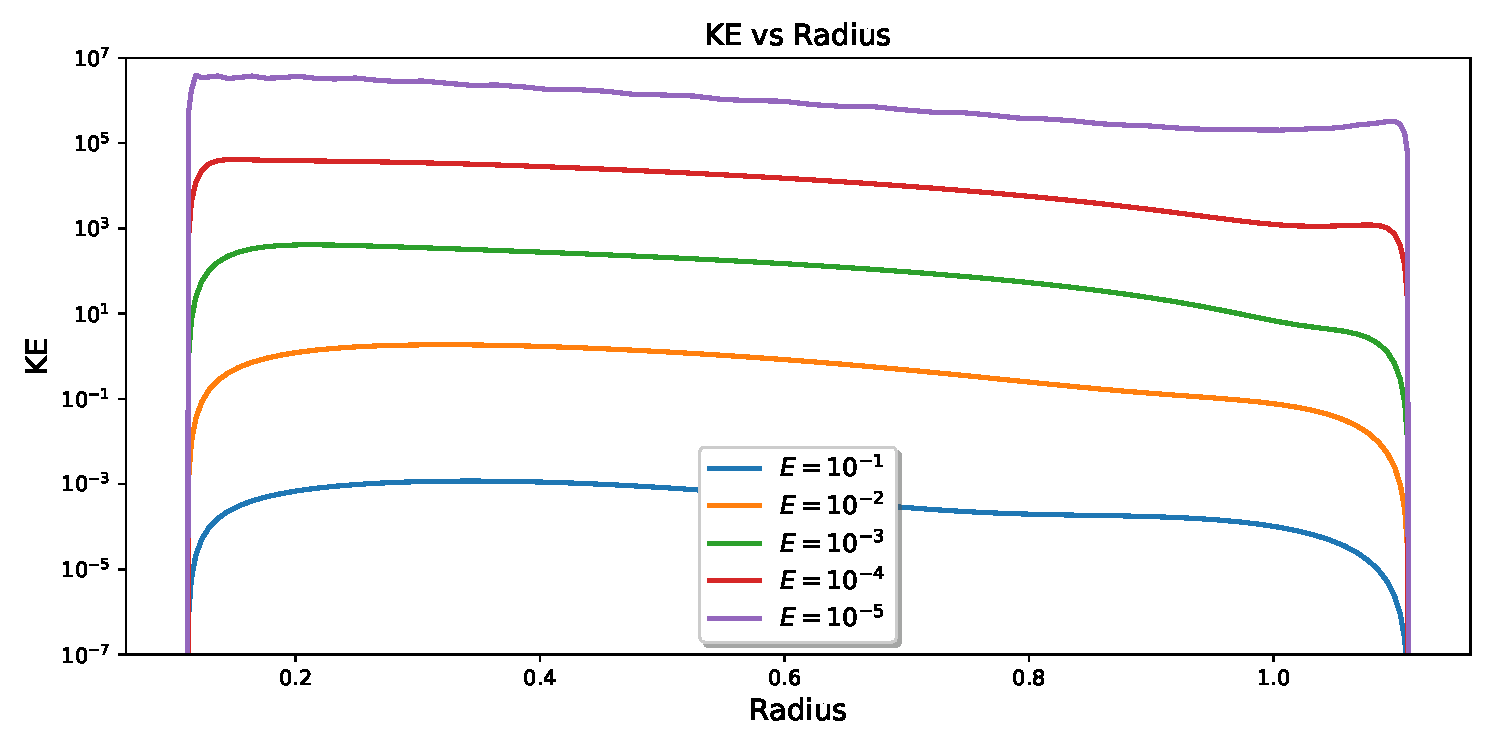
\includegraphics[width=1\textwidth]{figures/ke_radius_all.pdf}
    %\caption[Solar interior regions]{Visual representation of the three solar interior regions \cite{solarscience}.}
    \caption{Kinetic energy shell average as a function of radius during equilibrated phase for a range of Ekman numbers.}
    \label{fig:ke_radius}
\end{figure}
}


\def\azavgtemperature{
\begin{figure}[h]
    \centering
    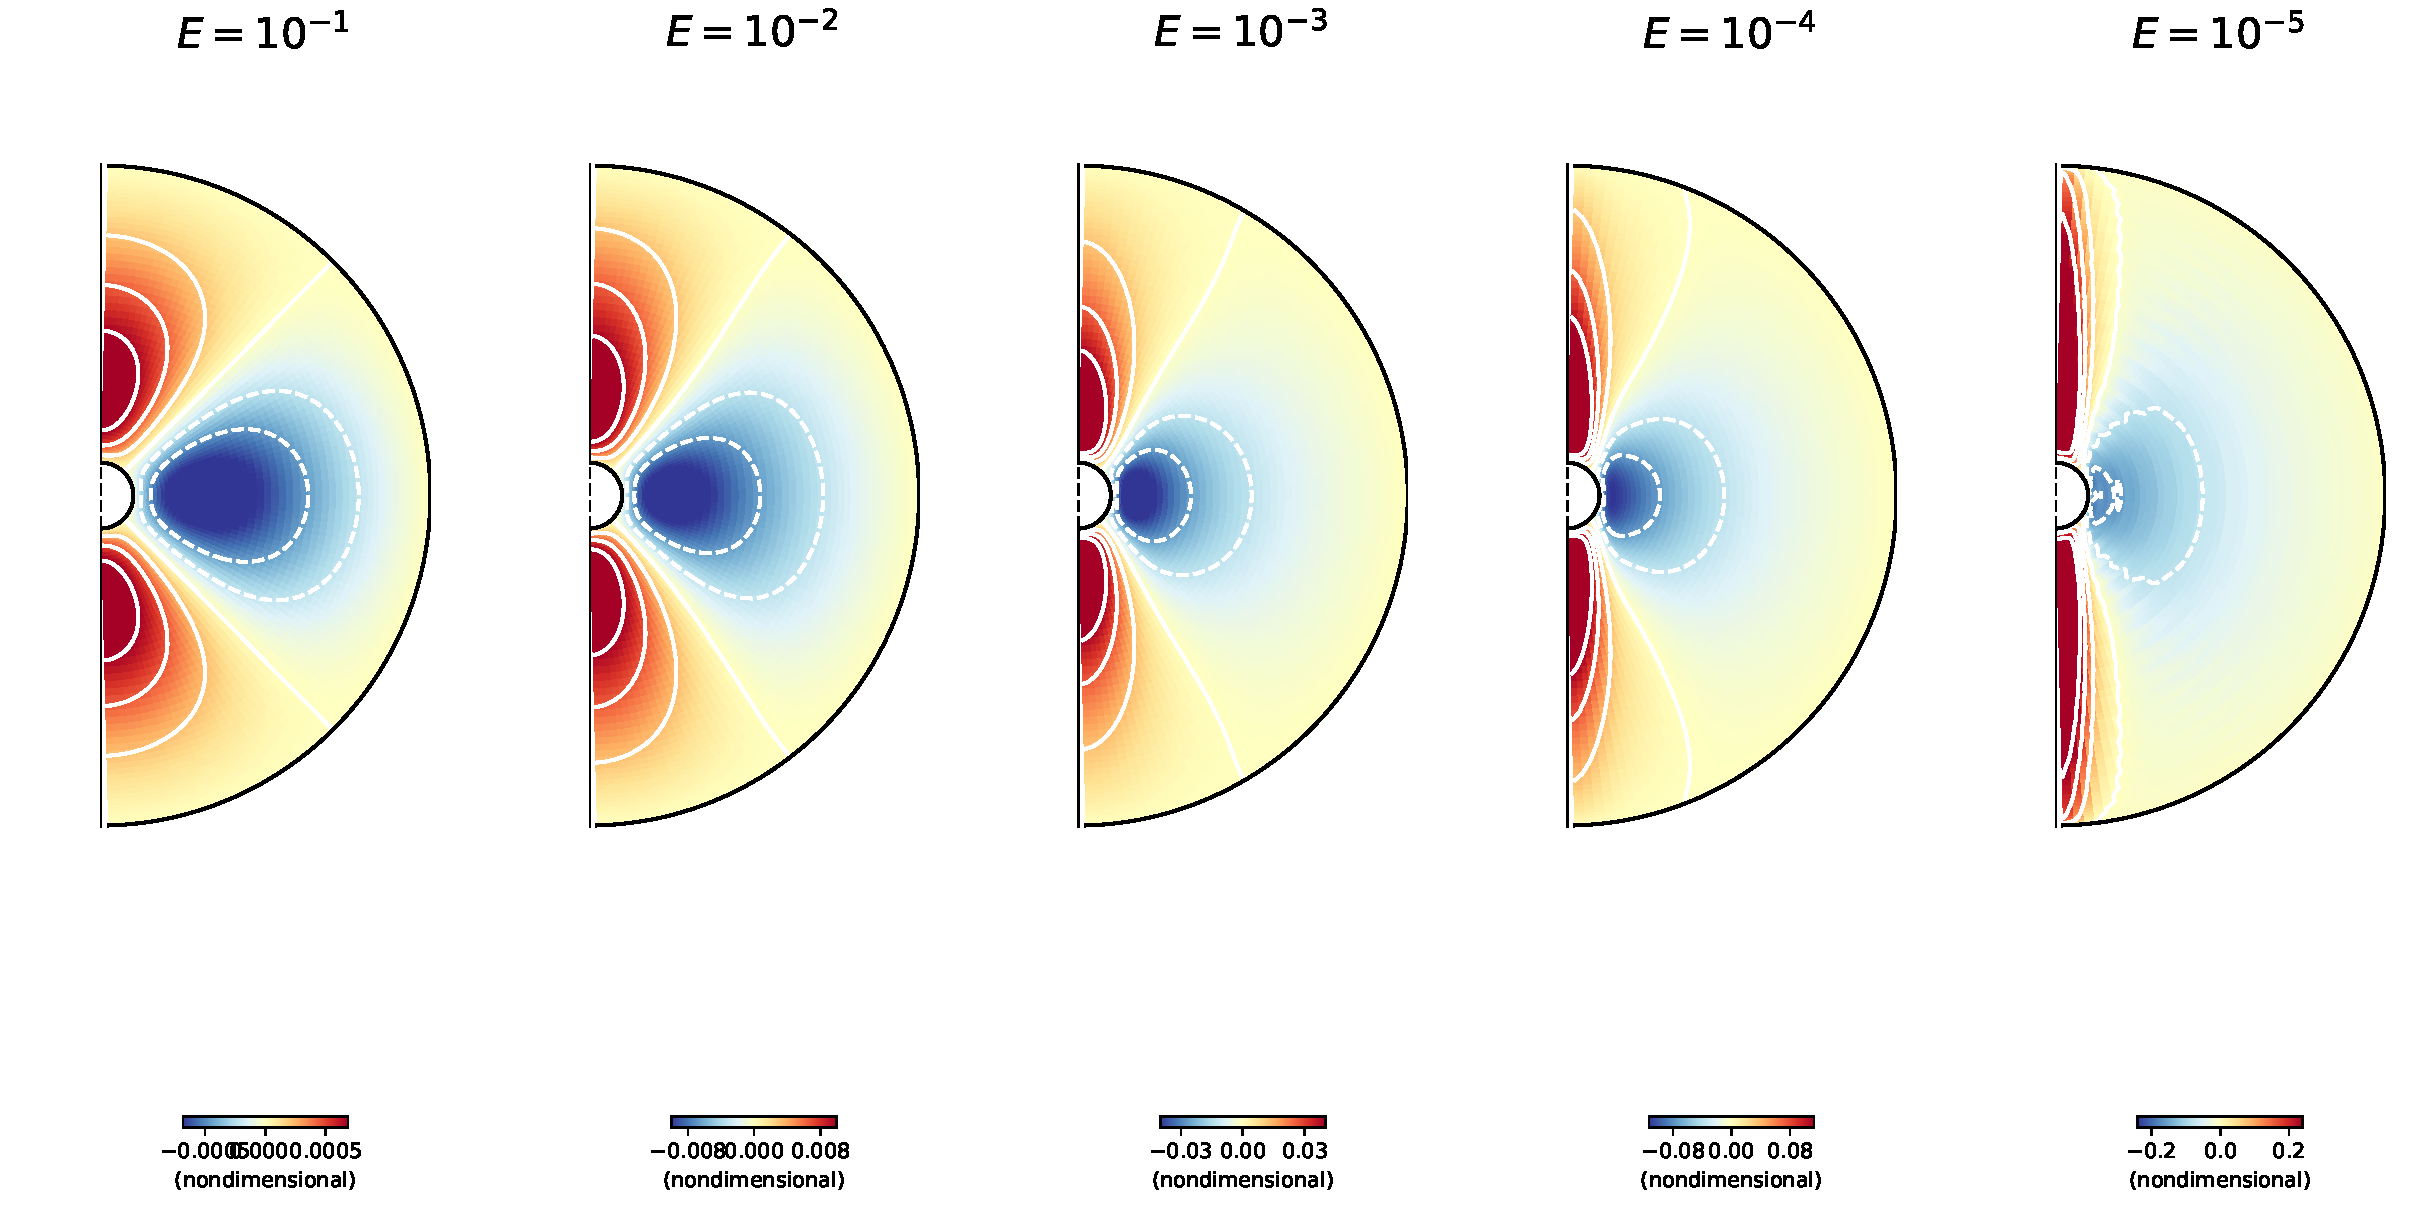
\includegraphics[width=1\textwidth]{figures/AZ_Avgs_501.pdf}
    %\caption[Solar interior regions]{Visual representation of the three solar interior regions \cite{solarscience}.}
    \caption{Temperature azimuthal average during equilibrated phase for a range of Ekman numbers.}
    \label{fig:az_avg_temperature}
\end{figure}
}

\def\azavgomega{
\begin{figure}[h]
    \centering
    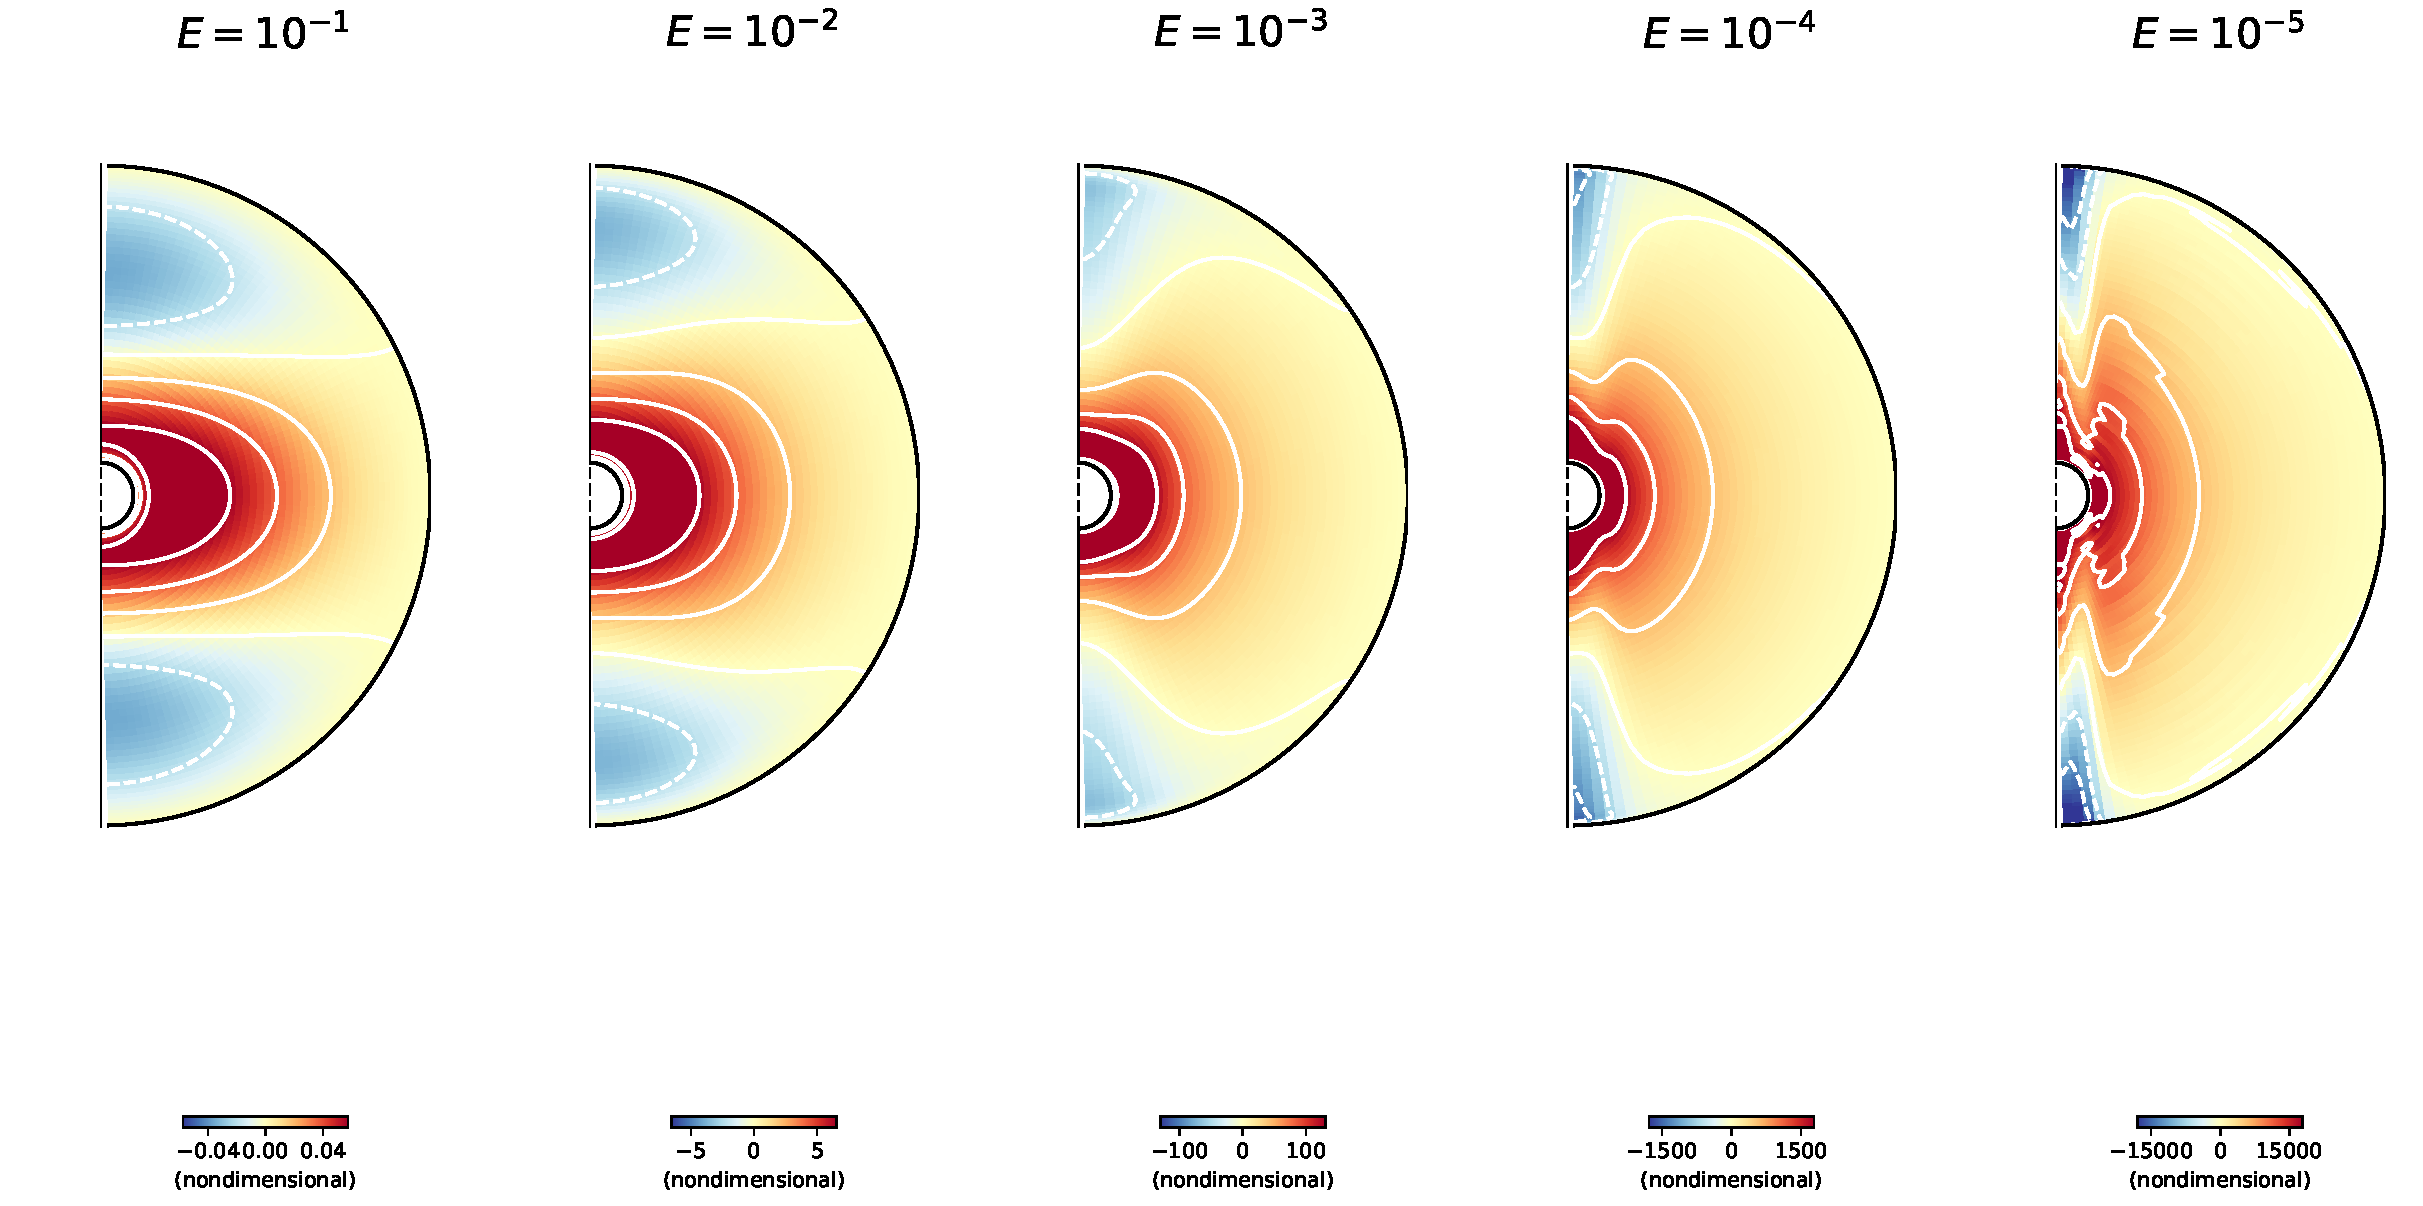
\includegraphics[width=1\textwidth]{figures/AZ_Avgs_omega.pdf}
    %\caption[Solar interior regions]{Visual representation of the three solar interior regions \cite{solarscience}.}
    \caption{Angular velocity azimuthal average during equilibrated phase for a range of Ekman numbers.}
    \label{fig:az_avg_omega}
\end{figure}
}

\def\azavgmassflux{
\begin{figure}[h]
    \centering
    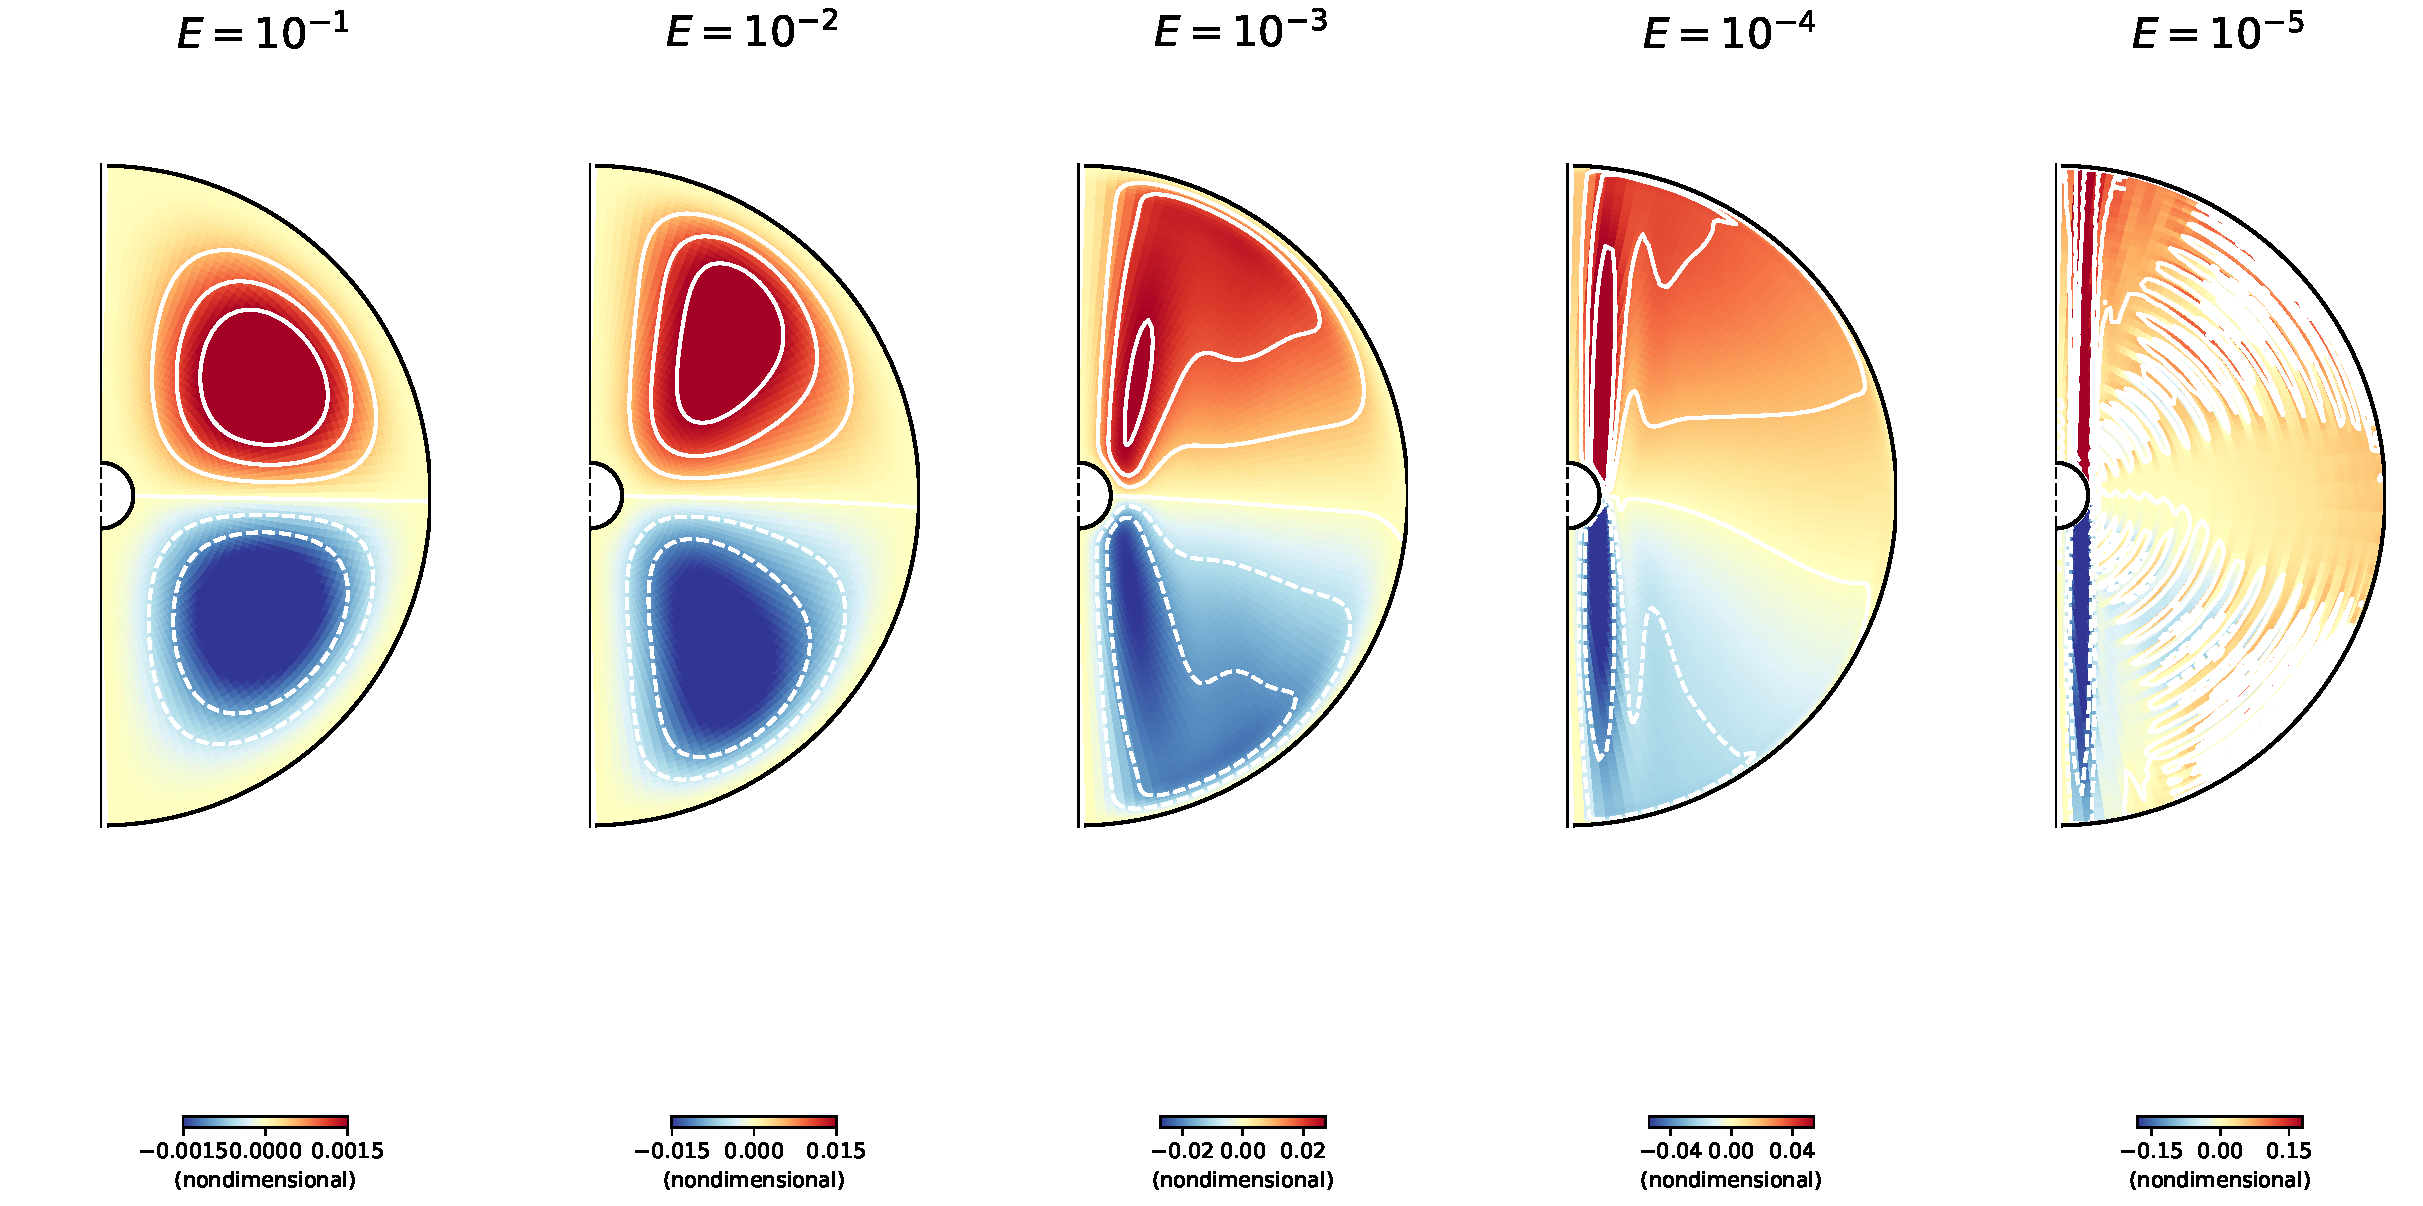
\includegraphics[width=1\textwidth]{figures/AZ_Avgs_massflux.pdf}
    %\caption[Solar interior regions]{Visual representation of the three solar interior regions \cite{solarscience}.}
    \caption{Mass flux azimuthal average during equilibrated phase for a range of Ekman numbers.}
    \label{fig:az_avg_massflux}
\end{figure}
}
